\documentclass{article}

\usepackage{listings}
\usepackage{color} %red, green, blue, yellow, cyan, magenta, black, white
\definecolor{mygreen}{RGB}{28,172,0} % color values Red, Green, Blue
\definecolor{mylilas}{RGB}{170,55,241}

\usepackage{graphicx}
\usepackage{subcaption}

\usepackage{float}

\usepackage{geometry}
\geometry{a4paper,margin=2.5cm}
\setlength{\parindent}{0pt} %no indentation between paragraphs
\setlength{\parskip}{4pt} %space between paragraphs

\title{CSSE7014 Distributed Computing \\
Assignment 2 \\
Semester 1, 2017}
\author{Paul Kogel (44644743), Ramdas Ramani (44743767), Andi Nuruljihad (44159069)}

\begin{document}

\maketitle

\pagebreak
\tableofcontents\thispagestyle{plain}

\pagebreak

\section{Introduction}

In the recent years, cloud computing has experienced an enormous boom: with resources like compute and storage provided as a service, developers have been able to create a completely new kind of applications. For instance, a computation-intense process such as text-to speech can now be provided on a resource-constraint mobile device, simply by delegating the majority of the computations to a cloud service.
%
%Main issues with cloud: delay (distancce + mobility), scalablity
As the number of devices requesting data from the cloud rises, and the Internet of Things (IoT), the inter-networking of everyday objects via the Internet, continues to expand, cloud services are facing the ever-growing challenge of scaling to accommodate the increasing number of objects transmitting and receiving data. In addition, with data centres often located hundreds of kilometres away from the user, keeping latencies low is also a challenge. While this might not be an issue in some use cases, applications like connected vehicles are expected to process great amounts of data in real time. If information about an upcoming red traffic light would be, for example, delayed by a second, the vehicle might fail to brake in time, causing great disaster. 

Fog computing, a new computing paradigm, is set to address these issues. Described as extension of cloud computing ``to the edge of the network'' \cite{bonomi2012fog}, it moves traditional cloud services like storage, networking and compute to devices that are closer to the edge \cite{cisco2015fogcomputing}. This not only enables location-aware services, but also dramatically helps reducing delays, and thus, make real-time applications possible. In addition, fog based systems also support large numbers of devices, so-called ``fog nodes'', that are possibly widely geographically distributed, and highly mobile. Network connections are mostly wireless, and the network itself is heterogeneous, consisting of different types of nodes \cite{bonomi2012fog}.

In this essay, we provide an overview of the emerging area of fog computing. In the first section, we present different architectures for fog-based systems. Then, in the second section, we discuss common issues associated with the fog in general. Finally, we illustrate the benefits of using the fog by giving three examples for real-world applications.

As fog computing is still a fairly new field, though, many details concerning concrete architectures, or implementation specifics remain open, and should therefore be considered content of future work.

\pagebreak
\section{Architectures and Models}

In this section, we are going to discuss different basic architectures that are commonly used in fog environments. Fog is still a developing field, and very broad, with many different use cases. To give good overview, we will present two specific architectures namely software-defined fog network architecture and gateway-based fog computing architecture.
We will then look at the efforts of the OpenFog consortium to provide a standardised framework for building fog applications.

\subsection{Gateway-based fog computing architecture}

Internet of Things (``IoT'') is a huge global information system composed of many objects that can be identified, sensed and processed based on standardized and interoperable communication protocols\cite{lee2016gateway}.
In general, most of the IoT services and applications, some of which are namely connected vehicle, smart grid, smart cities, and wireless sensors and actuators networks (``WSANs'') require mobility support, location awareness and low latency \cite{lee2016gateway}. 
These features are not readily realisable using the traditional cloud computing paradigm and that is where a computing model such as fog computing model that extends a traditional cloud computing model fits in.

One of the key elements of the IoT are wireless sensor networks where multiple heterogeneous wireless communications coexist: such as WiFi, ZigBee, cellular and Bluetooth. 
Wireless sensor networks are a collection of nodes that are used to sense and interact with the environment in which they are set up. Actuators however add a new dimension to sensor networks by bringing the ability to control the system. Some applications which require physical actions such as open, close, move and focus can use actuators to achieve them. Furthermore WSANs are still domain specific and usually deployed to support a specific application\cite{lee2016gateway}.   

Wangbong lee et al. \cite{lee2016gateway} propose a gateway-based fog computing architecture for WSANs. The fog computing setup consists of a set of gateways and a microserver \cite{lee2016gateway}.
The gateway and micro server are connected by an Ethernet interface and the interfaces between gateway nodes are a combination of wired and wireless interfaces such as 3G, LTE, and Ethernet\cite{lee2016gateway}.

Figure \ref{fig:gateway} shows the architecture both from a physical and logical view.

\begin{figure}
\centering
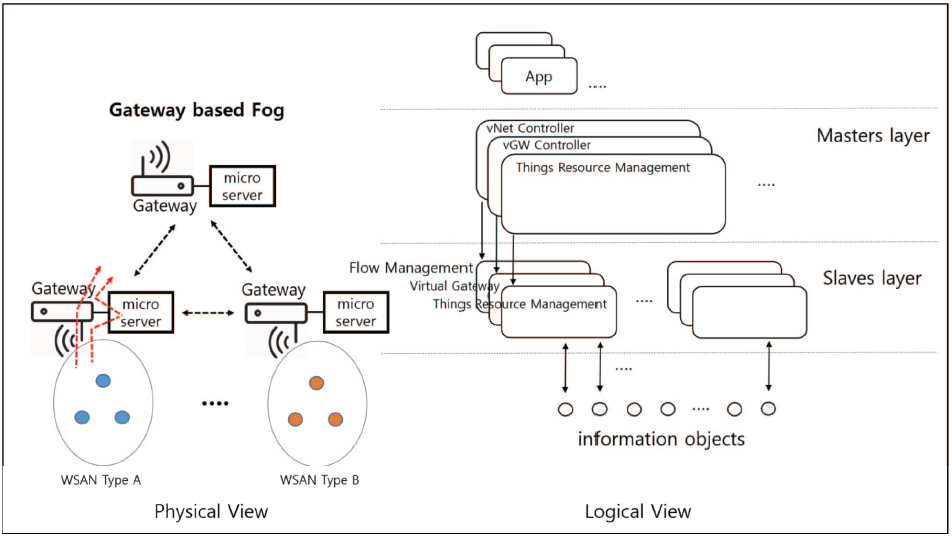
\includegraphics[scale=0.5]{gateway.png}
\caption{Gateway-based fog computing architecture for WSANs \cite{lee2016gateway}}
\label{fig:gateway}
\end{figure} 

The nodes can be seen as classified into slave nodes and master nodes. Slave nodes took care of functions such as flow management, virtual gateway and resource management whereas the master nodes have control over the functionalities of the slaves \cite{lee2016gateway}. The gateways have their own role where they function as a master/slave node. As shown in figure \ref{fig:gateway}, the slave nodes and master nodes exist in their respective layers when looked at from a logical point of view. 

Flow management for this setup is based on software defined network such as OpenFlow, and virtual function management needed a light version of NFV (Near Field View) architecture such as ClickOS \cite{martins2014clickos} which helps in network function virtualisation.
The architecture provided helps virtualize WSAN and the model is event driven. It provides virtual event from networked objects and shared them to various applications.

In order to understand why a fog computing setup is preferred, we need to look at the amount of data interchange that goes on in WSANs.
Latency of the application also plays a major role in applications involving WSANs (low latency is key) and it is desirable to make the applications function in real time.
This is not possible to realise in a cloud model where the latency is high. This could be attributed to the fact that the control topology of fog computing is distributed whereas cloud is centralized \cite{lee2016gateway}.
Furthermore, most important fog applications involve real-time interactions rather than batch processing \cite{lee2016gateway}. 
An example would be the large-scale sensors networks to monitor the environment. Since such a setup would inherently be distributed and require distributed computing and storage resources, fog computing with its large number of nodes as evidenced in sensor networks in general is preferred \cite{lee2016gateway}. 


\subsection{Software-defined fog network architecture for IoT}

Before we discuss the software-defined fog network for IoT, let us look at how a traditional IoT architecture looks and how it is realised.
Figure \ref{fig:iot} shows such an architecture from a a high-level perspective.

\begin{figure}
\centering
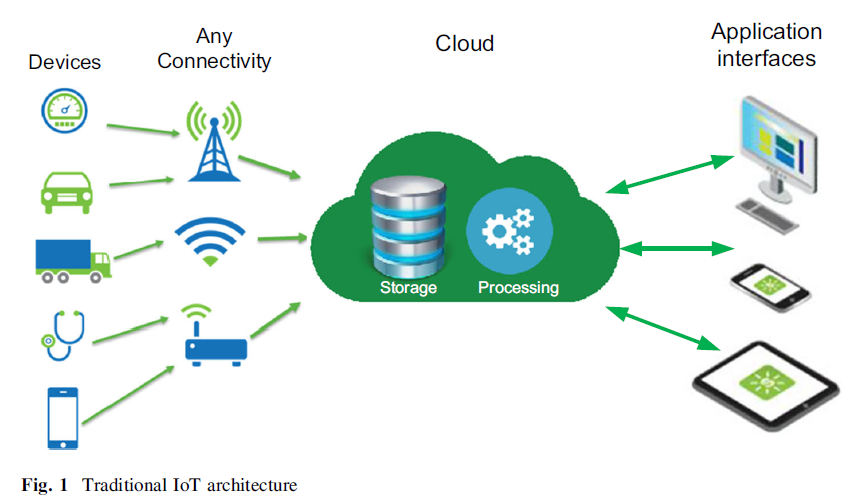
\includegraphics[scale=0.5]{iot.png}
\caption{Traditional IoT architecture \cite{tomovic2017software}}
\label{fig:iot}
\end{figure} 

Four main components are involved and they are \cite{tomovic2017software}: 
\begin{itemize}
\item Sensing devices or as we call them 'things'
\item Local communication network
\item The Internet Cloud
\item The Back-end IoT applications
\end{itemize}

The sensing devices collect/sense data from the physical environment which is then used in applications such as smart transportation to provide a desirable service to end customers. 
Since IoT devices are in general characterized by very limited memory and computational resources, IoT application usually take advantage of services offered by the cloud for data storage and processing. Furthermore, in order to reach the cloud, sensing devices rely on different communication technologies \cite{tomovic2017software}. 
Many emerging IoT applications require real-time interaction and mobility support (e.g. smart traffic lights and target tracking systems), which makes network latency an important limiting factor \cite{tomovic2017software}. Latency introduced in the network is not only a consequence of long distance between IoT devices and the cloud but its also caused by queuing delay, which is non-negligible on the congested links \cite{tomovic2017software}. 

In order to address these challenges, Slavica Tomovic et al. \cite{tomovic2017software} propose a model of IoT architecture which takes advantage of both the software-defined networking (``SDN'') and fog computing paradigms.
 
Novelty introduced with SDN as opposed to a traditional communications network is a clear separation of the control plane (signalling traffic, performing route calculation, system configuration and management) and the data plane (transport of packets to destination) \cite{tomovic2017software}. 
Here, the SDN control plane is placed on a logically centralized controller, which maintains a global view of the network, interacts with simple forwarding devices and provides a programming interface for network management applications \cite{tomovic2017software}. 
In this way, SDN allows network managers to configure and optimize network resources dynamically via automated programs \cite{tomovic2017software}.
 
The proposed architecture is intended to realise the IoT scenario where features of both technologies (SDN and Fog) are combined together in one integrated system.
The setup, shown in figure \ref{fig:sdn}, involves end devices with multiple wireless communication solutions, SDN controllers, heterogeneous fog infrastructure (virtualised servers, routers, access points, etc.) and cloud in the network core \cite{tomovic2017software}.

\begin{figure}[H]
	\centering
	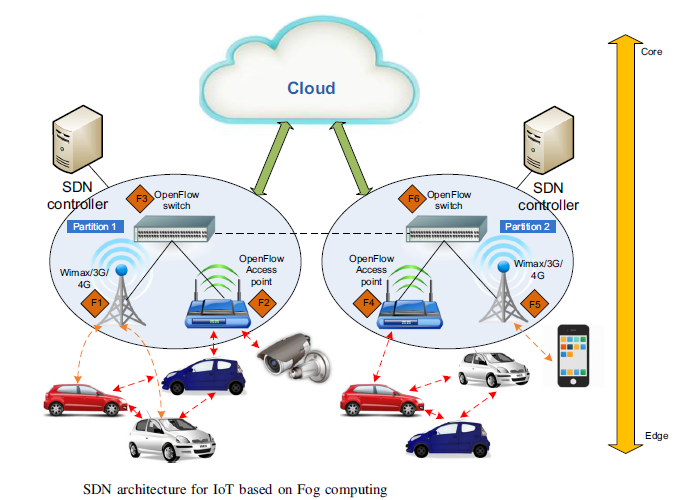
\includegraphics[scale=0.5]{sdn.png}
	\caption{SDN architecture for IoT based on Fog Computing \cite{tomovic2017software}}
	\label{fig:sdn}
\end{figure} 

The fog nodes expose a set of APIs for application deployment and development, resource management and control. Since IoT applications may in general be geo-spatially distributed, a hierarchical deployment of fog network was assumed. 
Mobile fog programming model \cite{hong2013mobile} is used in the development of IoT applications using hierarchically deployed and heterogeneous fog resources.
The final application consists of multiple processes that perform different tasks based on the device capability and position in the network hierarchy.

For example, tasks of large-scale video surveillance application are organized in three levels: motion detection at IP camera, face recognition at edge fog nodes and aggregation of identities at cloud server \cite{tomovic2017software}.

As discussed earlier, since IoT applications deal with dynamic workload due to periodic or event-driven data delivery models, they should be transparently scaled at runtime. In other words, there should be no issues with contention of resources upon scaling. 
In order to achieve that, Slavica Tomovic et al. \cite{tomovic2017software} propose logical centralization of orchestration functionality at the SDN controller.
To achieve that, they modify the design of SDN controller to perform the following functions:

\begin{itemize}
	\item Fog Orchestration 
	\item Spread routing logic into SDN-enabled network elements
	\item Optimally select access points for IoT devices
\end{itemize}

In order to perform the above tasks, the controller collected and maintains information about fog nodes such as available memory, storage, running operating systems, software applications, state and interconnectivity of the network elements and characteristics of the connected smart devices.
The fog orchestration is then performed according to the business policies defined by the application service providers and the policies were stored in the SDN controllers and the fog nodes hosting the provider's application \cite{tomovic2017software}.

SDN controller therefore provides dynamic, policy-based management of fog services. It can track mobile devices and predict their potential destinations in the near future \cite{tomovic2017software}. This enables seamless handover to a new fog node at the network edge which would otherwise not be possible using a traditional cloud because of its centralised topology.

Besides fog orchestration, SDN controller also performs traffic control and connectivity management for IoT devices.
Another main component that is introduced in the architecture us a software OpenFlow switch. 
The application traffic always passes this component before being sent, which allows the control plane elements (i.e. fog nodes at the edge and SDN controllers) to identify the access of traffic flows into the network \cite{tomovic2017software}. 

Important use cases of such a system would be smart transportation, video surveillance etc. where low latency and real-time streaming takes preference. Besides fog computing, the presented system model can also exploit benefits of SDN to dynamically assign higher priority to some traffic flows in emergency situations, and hence guarantee low-latency.

\subsection{OpenFog Reference Architecture}

The OpenFog Reference Architecture (OpenFog RA) is the product of the OpenFog Architecture Workgroup, co-chaired by Charles Byers (Cisco) and Robert Swanson (Intel), and represents the collaborative work of the global membership of the OpenFog Consortium \cite{openfogconsortium2017}. The OpenFog Consortium was formed in November 2015 and is based on the principle that an open fog computing architecture is necessary in today’s increasingly connected world \cite{openfogconsortium2017}.

The main idea behind the OpenFog RA is to help business leaders, software developers, silicon architects, and system designers create and maintain the hardware, software and system elements necessary for fog computing and provide a medium to high level view of system architectures for fog nodes and networks \cite{openfogconsortium2017}.

The OpenFog RA describes a fog platform that is generic and can be designed to be fit any vertical market or application. 
This architecture is applicable across many different markets including, but not limited to, transportation, agriculture, smart-cities, smart–buildings, healthcare, hospitality, financial services, and more, providing business value for IoT applications that require real-time decision making, low latency, improved security, and are network-constrained \cite{openfogconsortium2017}.

The OpenFog RA is driven by a set of core principles called pillars \cite{openfogconsortium2017}.
The pillars can be thought of as the key attributes that a system needs to adhere to to embody the OpenFog definition of a horizontal, system-level architecture that provides the distribution of computing, storage, control, and networking functions closer to the data source \cite{openfogconsortium2017}.

The Pillars \cite{openfogconsortium2017} are:

\begin{itemize}
\item Security - Security in the OpenFog RA describes all of the mechanisms that can be applied to make a fog node secure. 

\item Scalability - Since the hierarchical nature of fog adds scaling opportunities, this pillar addresses the dynamic technical and business needs behind fog deployments. Because of the variability in the use cases for fog computing, the OpenFog RA enables elastic scaling based on demand \cite{openfogconsortium2017}.

\item Openness - Openness as a basic principle enables fog nodes to be present anywhere in a network and span across networks thereby enabling pooling by discovery, which means that new software-defined fog nodes can be dynamically created to solve a particular scenario \cite{openfogconsortium2017}.

\item Autonomy - This pillar enables fog nodes to continue to deliver their intended functionality in the face of external service failures. In this architecture, autonomy is supported throughout the hierarchy and therefore decision making will be made at all levels of a deployment’s hierarchy including near the device or higher order layers. It does not rely upon a centralized system for operation (e.g. a backend cloud) \cite{openfogconsortium2017}.

\item Programmability - This pillar enables highly adaptive deployments including support for programming at the software and hardware layers. This means re-tasking of a fog node or a cluster of fog nodes can be completely automated \cite{openfogconsortium2017}. The fog nodes' inherent programmability interfaces are made use of in such a case.

\item Reliability, Availability and Serviceability (RAS) - Hardware, software, and operations are the three main areas of the RAS pillar and as such take on great importance in the OpenFog RA \cite{openfogconsortium2017}.

A reliable deployment will therefore continue to perform as expected under all conditions. Availability ensures continuous management and orchestration, which is usually measured in uptime, while servicing a fog deployment ensures correct operation.

\item Agility - This pillar addresses the business operational decisions for an OpenFog RA deployment. It also deals with the highly dynamic nature of fog deployments and the need to respond quickly to change\cite{openfogconsortium2017}.

\item Hierarchy - This pillar ensures that the OpenFog RA is complementary to traditional cloud architectures. Depending on the scale and nature of the scenario being addressed, the hierarchy may be a network of smart and connected partitioned systems arranged in physical or logical layers, or it may collapse into a single physical system (Scalability pillar) \cite{openfogconsortium2017}.
\end{itemize}  

\subsubsection{OpenFog RA Description - Views and Perspectives}

The OpenFog RA Description is a composite representation of various stakeholder concerns which are referred to as ``views'' \cite{openfogconsortium2017}. The stakeholders and their associated views are identified because they are required to facilitate any successful fog based deployment \cite{openfogconsortium2017}. 

The functional viewpoint of the architecture describes how the OpenFog architectural elements and views are applied to satisfy the stakeholders' requirements/concerns on a given scenario. It is, however, important to note that these change over time. 

The deployment viewpoint addresses how the fog software and fog systems are deployed in order to satisfy a given stakeholder scenario. The deployments generally happen in a hierarchy-based model where the number of tiers are dictated by the scenario requirements \cite{openfogconsortium2017}. The scenarios might be the amount and type of work required by each tier or the number of sensors required for the deployment and so on.

The abstract architecture comprising the views and perspectives is shown in figure \ref{fig:openfog_ra}.

\begin{figure}[H]
	\centering
	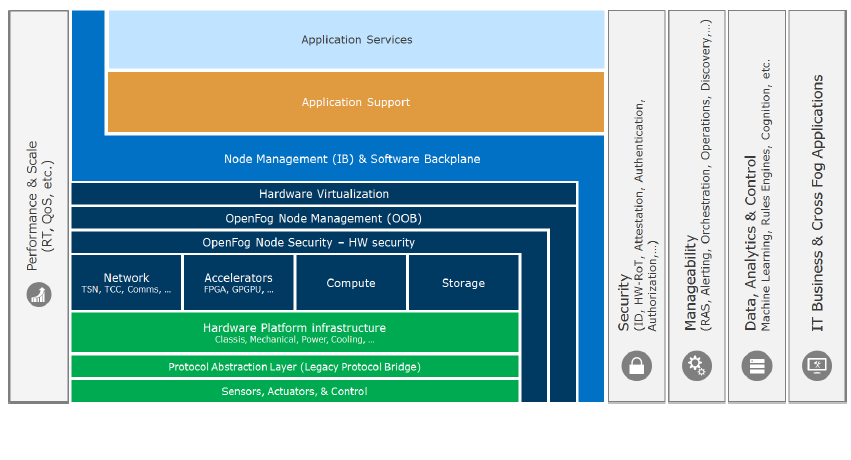
\includegraphics[scale=0.5]{figa.png}
	\caption{Architecture description with perspectives \cite{openfogconsortium2017}}
	\label{fig:openfog_ra}
\end{figure} 

The grey vertical bars on the sides of the views are referred to as ``perspectives'' \cite{openfogconsortium2017}. They can be thought of as concerns that are to be employed in the fog implementation. The reference architecture features the following perspectives:

\begin{itemize}
\item Performance - This is an important concern, also referred to as a ``cross-cutting concern'', as it impacts system and deployment scenarios, e.g., low latency.

\item Security - Data integrity is a special aspect of security for devices that currently lack adequate security. This includes intentional and unintentional corruption \cite{openfogconsortium2017}.

\item Manageability - Managing all aspects of fog deployments, which include RAS, DevOps, etc. \cite{openfogconsortium2017}. 

\item Data Analysis and Control -  The autonomy of fog nodes requires localized data analytics coupled with control \cite{openfogconsortium2017}.

\item IT Business and Cross-Fog Applications - Ability to migrate and operate properly at any level of a fog deployment’s hierarchy \cite{openfogconsortium2017}.  
\end{itemize}

The views (representations of stakeholder concerns) \cite{openfogconsortium2017} described in the OpenFog RA description include:

\begin{itemize}
\item Software View - Represented in the top 3 layers shown in Figure \ref{fig:openfog_ra} and includes application services, application support, node management (IB) and software backplane \cite{openfogconsortium2017}.

\item System View - Represented in the middle layers shown in Figure \ref{fig:openfog_ra} and includes hardware virtualization down through the hardware platform infrastructure \cite{openfogconsortium2017}.

\item Node View - Represented in the bottom layers shown in Figure \ref{fig:openfog_ra} and includes the Protocol Abstraction Layer and sensors, actuators, and control \cite{openfogconsortium2017}.
\end{itemize} 

\subsubsection{OpenFog Reference Architecture Deployment Models} 

In most fog deployment models, there are usually tiers (N-tiers) of nodes. Depending on the particular use case, multiple fog and cloud elements may collapse into a single physical deployment. Each fog element may also represent a mesh of peer fog nodes in use cases like connected cars, electrical vehicle charging, and closed loop traffic systems \cite{openfogconsortium2017}.

\begin{figure}[H]
	\centering
	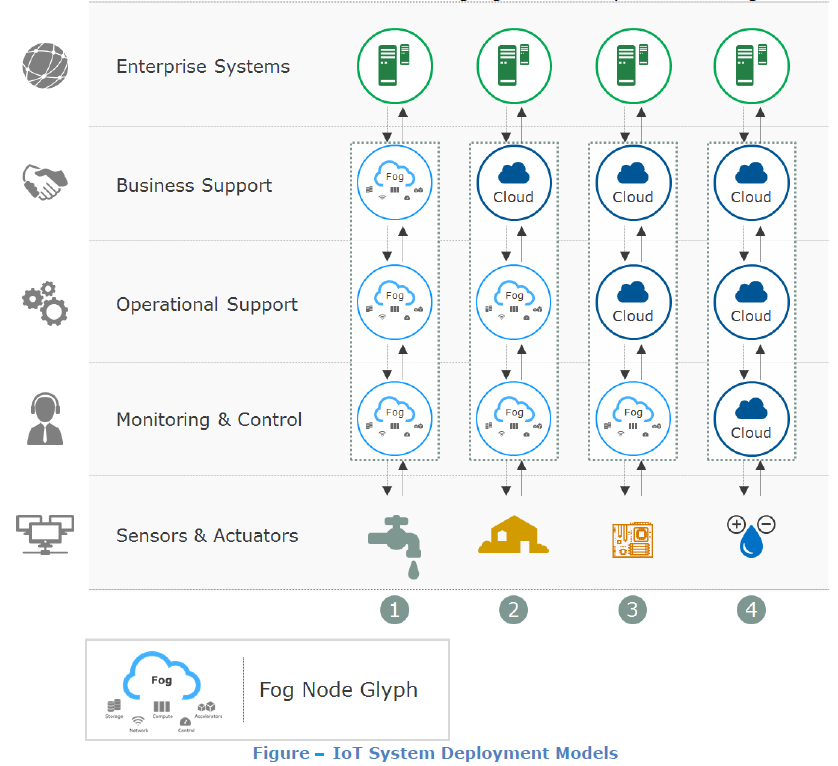
\includegraphics[scale=0.5]{models.png}
	\caption{IoT system deployment models \cite{openfogconsortium2017}}
	\label{fig:depl_models}
\end{figure}

Figure \ref{fig:depl_models} provides an overview of different commonly-used deployment options. These options are:

\begin{itemize}
	\item Fog Model Independent of the Cloud - This model is mainly used in cases where cloud services can't be used. The reasons might be response-time concern, compliance to regulations, security and privacy, or unavailability of a centralised cloud.
	
	Use cases include armed forces combat systems, drone operations, some healthcare systems, hospitals, and ATM banking systems \cite{openfogconsortium2017}.

	\item Model using Cloud for Business Support - This model uses the cloud for business support (information processing related to decision making).  However, the actual operation-centric information processing is done by fog deployments located close to the infrastructure/process being managed.

	Use cases include commercial building management, commercial solar panel monitoring, and retail \cite{openfogconsortium2017}.

	\item Model using Cloud for Business and Operational Support - This model uses local fog infrastructure for time-sensitive computation, while the cloud is used for the balance of operational and business-related information processing.

	Use cases include commercial UPS device monitoring, mobile network acceleration, and content delivery networks (CDNs) for Internet acceleration \cite{openfogconsortium2017}.

	\item Model using Minimal/No Fog Infrastructure - This model leverages the cloud for the entire process due to the environmental constraints which would make the deployment of fog uneconomical or infeasible.

	However, fog nodes that are at the lowest level (device layer) may be designed with monitoring and control functions for safety related control.

	Use cases include agriculture, connected cars, and remote weather stations \cite{openfogconsortium2017}
\end{itemize}


\pagebreak

\section{Common Issues}
% Comments on issue related to communication paradigms, fault tolerance, consistency, reliability, etc.
% Marking criteria: Quality discussion and explanation on relevant issues as required with clear examples. Discussions of potential enhancement to address any performance issues are provided.

Though still an emerging field, previous research, such as Yi et al.'s ``survey on fog computing'' \cite{yi2015survey}, has been able to identify multiple potential issues related to fog computing. In this section, we summarise their main findings, and provide additional discussion and research related to them whenever possible.

To improve clarity, we organise issues around 5 main areas: networking, optimal use of resources, fault tolerance, application development, and security and privacy. Note that we focus purely on technical issues. Business-related aspects, such as implementation of a viable business model, and billing mechanisms, are not covered.

\subsection{Networking}
In order for the fog to function properly, the network has to provide nodes with connectivity, and additional network services, such as routing. The particular nature of the fog, though, makes the implementation of these functions difficult. 

For example, the network has to be highly scalable, providing support for a large number of potential nodes. In addition, it should be able to cope with constant topology changes caused by node mobility.

Using virtualisation mechanisms, such as SDN, has been deemed as viable solution to these issues \cite{yi2015survey}. In their proposal of a general architecture for the fog, Bonomi et al. \cite{bonomi2014fog} state that the fog should use virtualisation for ``key resources'', including networking. An architecture based on SDN is described in the architecture section. Using SDN, however, might not always be an option, as the as it puts ``a high emphasis'' \cite{peng2016fog} on a centralised architecture, with a small number of ``SDN controllers'' in charge. This basically creates a single point of failure: if the controllers cannot be reached, e.g. due to unreliable network links, the system is not able to function properly. To make the network more robust, a decentralised model as described by \cite{yi2015survey} might be used, where  ``each node should be able to act as a router for nearby nodes''. 

\subsection{Optimal resource use}
\label{sub_opt_res_use}

As stated before, the fog is highly heterogeneous. This heterogeneity is greatly reflected by different degrees of resource availability throughout the system. Important resources are storage, computation power and bandwidth. For example, in parts of the system, available bandwidth might be high due to the presence of more powerful network links, while in others, it can be a scare resource.

Naturally, these resources should be ``optimally'' used. However, the actual optimisation goal is highly dependent on the use case: for example, in a real-time application, the main objective is to ensure a small delay. Using more bandwidth or computation power to meet this goal is a valid trade-off. For a computation-heavy application running on a mobile device, in contrast, reducing the amount of computation performed locally on the device might be most important.

In their paper, Yi et al. \cite{yi2015survey} present several strategies that might be used to optimise resource use under different circumstances. 
%
Firstly, they suggest that the adequate placement of data can help optimising bandwidth use. In the previously given example of a real-time application, storing data on nodes that are well-connected to the consumer could significantly reduce delay. This placement, however, has to take the dynamic nature of the fog into account. If a node changes location, for example, data placement on the same node can result in small latencies at one time, but introduce great delays at another time. Even if the location of the consumer does not change, available bandwidth at a link might, e.g. if more nodes are interested in the data.
%
Besides placing data, the authors also suggest to place computation. Using ``computation offloading'', an operation can be partly or fully delegated to a different node in the network. In the aforementioned example of the computation-heavy application, for instance, a more powerful node could perform most of the computation-intense work. Determining which parts of the computation to offload to which nodes, though, can be challenging. As for data placement, this is largely due to the dynamic nature of the fog.
%
Lastly, they present different methods based on the concept of adjusting the network topology. For example, they suggest that effectively choosing the relay nodes for one or multiple endpoints could help reducing delay, while increasing throughput. Again, however, constant changes in the environment, especially the topology, make an implementation challenging.

Focusing less on choosing locations for data and operations, and more on resources actually available at a given node, Aazam and Huh \cite{aazam2015dynamic} present a resource management method that has been developed especially for the dynamic environment of the fog. At its core, their method predicts the resources required by a consumer for the use of a specific service, and uses these predictions to give ``guarantees'' about resource availability. For example, a consumer might get a guarantee of 80\% availability for a particular service, meaning that it will have access to all resources required to run the service for most of the time. Predictions are largely dependent on past consumer behaviour. If the node in the previous example had, for instance, frequently disconnected from the service provider, its resource guarantee would be lower. Basically, this means that if not sufficient resources are available, they would preferably be given to nodes that make better use of them. As it can be easily seen, this makes resource allocation considerably fair.

\subsection{Fault tolerance}
As describe before, the fog mainly uses unreliable wireless network links. In addition, nodes are highly mobile. Being able to ensure availability of services, and provide reliability in general are therefore important aspects.

To improve service availability, Yi et al. \cite{yi2015survey} suggest to adjust the network topology (see section \ref{sub_opt_res_use}). For instance, they present the idea of dividing a network into several clusters, with each cluster centred around a ``rich-resource'' node.

Traditionally, reliability in a distributed system can be provided by the means of techniques such as checkpointing or rescheduling (see \cite{tanebaum2013}). According to Yi et al. \cite{yi2015survey}, though, most of these techniques are unfit for the fog, as they introduce too much delay. They conclude that replication might work, but they expect it to be difficult to implement due to the distributed nature of the system. Additional research on the topic does not seem to exist. Madsen et al. \cite{madsen2013reliability} claim to provide such, but fail to give any actual fog computing-related insights.

%"However, taking a checkpoint is often a costly operation and may have a severe performance penalty." (p. 364)


\subsection{Application Development}
As stated in the introduction, the fog is dynamic in regards to network topology, and resource availability. In addition, fog nodes might run on different platforms and system architectures \cite{yi2015survey}. Developing applications that are able to run in this environment, and provide high compatibility, can be expected to be difficult. 

To ease development, Bonomi et al. \cite{bonomi2014fog} propose a ``fog abstraction layer'' that hides the underlying heterogeneity, and provides developers with a ``uniform and programmable interface''. Yi et al. make a similar suggestion by calling fr a ``unified interfacing and programming model'' \cite{yi2015survey}.

Due to issues mentioned in the beginning, though, we expect that the implementation of such a layer is challenging.

%TODO: what about cisco?

\subsection{Security and Privacy}
Many applications that have been proposed for fog computing are safety-critical, and/or process sensitive data. For example, in vehicle-to-vehicle communication, an insecure system that allows attackers to remotely control the car could have disastrous consequences. In home automation, users might be worried about giving third parties insights into their daily routine.

%Authentication/access control
Stojmenovic and Wen \cite{stojmenovic2014fog} find that providing authentication throughout the system is one of the ``main security issues'' for fog computing. As an example, they describe a smart meter that is modified by a user, and reports then, due to a lack of proper authentication, false readings. As a possible solution, they suggest encryption at node-level. For this, the meter would encrypt its data, and another node would decrypt it before further forwarding the data. Similarly to this, the OpenFog consortium deems access control (to which it counts authentication) as ``key to building a secure system'' \cite{openfogconsortium2017}. 

%Root of trust
In addition to advocating access control, the consortium's reference architecture for fog computing also defines a hardware component called ``root of trust'' that is ``at the heart of the [...] security of the fog node''. This component is tamper proof, and required to be implemented by every fog node. It provides security by creating a ``chain of trust'', i.e., selecting other components such as hardware, software, or other nodes that it considers trustworthy. If a component is compromised, like the smart meter in the example above, it would not gain trust from the root, and therefore not do any harm.
%stresses the importance of providing ``end-to-end security'' in general. To establish that, it

Though access control and the chain of trust promise to provide a solid foundation to a secure fog system, they are both rather general methods. In order to improve security in a given context, it has been suggested in \cite{openfogconsortium2017} to select additional measures based on the specific use case.

To protect privacy, Yi et al. \cite{yi2015survey} suggest to run ``privacy-preserving'' algorithms before data is transferred from the fog to the cloud. As examples, they mention techniques based on differential privacy and homomorphic encryption. Gerla \cite{gerla2012vehicular} makes an interesting point by stating that moving processing from the cloud to mobile devices alone gives users more control over their data. It can be easily seen, however, that this requires the implementation of adequate control mechanisms. The aforementioned reference architecture \cite{openfogconsortium2017} vaguely describes ``privacy attributes'' that a user can assign to his/her data, suggesting that these might be used to control its use.

\pagebreak

\section{Applications}
%Various examples (across different disciplines) provided with clear arguments why they are relevant.

Fog computing was conceptualized as an extension of the cloud to address services and applications for which the cloud paradigm is not entirely suitable \cite{bessis2014big}. As a relatively new model, the potential applications and likely infrastructure and design challenges for the fog are still being explored. However, there is a wide range of possible uses of a paradigm that enables real-time, low-latency processing, reduces bandwidth costs, with the benefits of improved security and governance. This section will detail some possible applications of fog computing in various fields.

\subsection{Real-time Health Monitoring}
Wireless Body Area Networks (WBAN) is an important technology in healthcare IoT applications that allows for the unobtrusive monitoring and recording of various vital signs of a patient in real-time. In current cloud-enabled health-monitoring systems, these WBAN devices are in a state of constant connection with a cloud server, sending patient health data to the cloud around the clock \cite{gia2015fog}. However, all of this data being transmitted and received by so many devices on a network can lead to high network bandwidth usage, and consequently, high latency and slow response times from the health monitoring system. In addition, proper analysis can only be performed after relevant data from all WBAN devices in a patient is received by the system. With each individual WBAN transmitting its raw data to the cloud via Wi-Fi, bottlenecks in the analysis might be caused by any single device that is slow or fails to upload data \cite{gia2015fog}. A small dip in the vitals of a patient on life support can quickly turn into a full-on drop within minutes, thus a model that can effectively and reliably monitor this health data in real-time is absolutely critical.

Gia et al., in a case study exploring a practical application of fog computing for WBAN health data feature extraction,  suggest the ``provision of an extra layer in between a conventional gateway and a remote cloud server''\cite{gia2015fog}. This added layer, described as the ``fog layer'' in the study, is essentially a fog gateway that pre-processes health data from the various sensor nodes, reducing the volume of data transmitted to the cloud and expediting the response time of vital applications as a result. As detailed in the study, instead of hundreds of WBAN devices each sending patient health data directly to a cloud server, the WBAN data is sent to a fog gateway. The fog gateway aggregates all of the WBAN data and groups together data that is relevant for each user. The gateway then pre-processes this data, storing recent results in a distributed fog database where it may be accessed by the patient or their doctor as permitted by the hospital. The pre-processed data is then sent to the cloud server for storage and to be related to data from other patients.

The fog computing model proposed by Gia et al. showcases how fog computing extends the cloud to allow for vital processes to be executed much closer to the edge. Since the raw WBAN data is collected and pre-processed at the fog layer, the number of devices communicating with the cloud is cut down from several hundred WBAN devices to a single fog gateway. As a result, the volume of data transmitted by the system is drastically decreased, affecting overall latency and response time. The model proposed in the study successfully reduced the size of data being sent to the cloud by at least 93\% while reducing latency more than 48.5\% in busy Wi-Fi networks \cite{gia2015fog}. 

\subsection{Security and Surveillance}
Surveillance and security camers generate massive volumes of data; a single camera may create over one terabyte of high-definition video data per day \cite{openfogconsortium2017visualsecurity}. An effective security system would require several security cameras in a number of locations for maximum coverage. In a cloud-based deployment, each of these cameras would be sending large volumes of video data to a cloud server at a remote location. This puts a great strain on the network, effectively forcing the system to dedicate a significant portion of its bandwidth solely for video transmission, resulting in significant latency. Security decisions must be made rapidly as situations may arise where a delay in response can result in a risk to public safety. If a person carrying a suspicious package is discovered on a camera, the system must be able to reliably track the package's movements. Delays in the system can result in out-of-date information being relayed to emergency services, making a timely response impossible.

The OpenFog Consortium released a paper proposing a fog computing model that may serve as a solution for this scenario \cite{openfogconsortium2017visualsecurity}. The paper recommends the deployment of fog nodes that can be designed to intelligently partition video processing between the various edge devices and the cloud. In contrast to traditional cloud models, this design allows video analytics to be performed at fog nodes that are physically close to the site, reducing latency and allowing for quicker response times in emergency situations. Relevant data can then be sent to the cloud to allow for historical analysis over long periods of time and enable data sharing between multiple locations \cite{openfogconsortium2017visualsecurity}, for example, the sharing of data between airports or multiple locations of a hotel chain.

The addition of an extra layer between the edge and the cloud allows for added security protocols to be implemented at the fog gateways where the raw camera data is processed before being sent to the cloud. This raw camera data is analyzed at the fog gateways, where rules may be established to determine which data should be sent to the cloud and which should be stored locally for security analysis purposes \cite{openfogconsortium2017visualsecurity}.

\subsection{Smart Cities - Traffic Congestion Management}
Traffic management is an ever-growing challenge faced by major cities; lost worker productivity, slower response times from emergency services, and high carbon emissions can all be attributed to traffic congestion. Various factors that contribute to traffic congestion simply can not be predicted, such as accidents. Even the predictablity of how certain weather affects road conditions can vary wildly between different areas. Furthermore, traffic management spans multiple jurisdictions; the development and implementation of potential solutions will probably take place in isolation within each department, hindering information sharing and integration initiatives \cite{openfogconsortium2017trafficmanagement}.

According to the OpenFog Consortium, proposed cloud solutions in Smart Cities, while suggesting a single cloud that connects these many departments, in reality involve multiple clouds for traffic management \cite{openfogconsortium2017trafficmanagement}. The paper notes that these departments are each responsible for the implementation of their own solutions to the traffic congestion problem for areas under their jurisdiction and, as a result, may potentially work with any number of clouds. This segmented approach, where each piece of the solution is developed and deployed in isolation, can result in the accumulation of redundant data and is an obstacle to data sharing between departments which in turn creates delays in response.

In a paper published by the OpenFog Consortium, a fog-enabled model is proposed to solve these problems \cite{openfogconsortium2017trafficmanagement}. CCTV, camera, electronic signage, and traffic light data will be captured by roadside or local fog nodes to be analyzed and used locally. These local fog nodes process this local data and transmit emergency messages (such as flooding or roadblock notices) at the local level. This local information would then be sent to a regional fog node where it would be related to data from other local fogs to piece together a picture of traffic conditions at a larger scale. These fog nodes at the regional and city level may be used to share information across individual networks, allowing for all relevant departments to share a single, synchronized picture of road-side conditions as they change. In the future, as manufacturers install fog nodes in their vehicles, each vehicle could potentially function as an edge device that connects with other devices on the road. All of this data in aggregate can be used by municipalities to provide a far more detailed view of traffic conditions, allowing for greater control of road conditions and much quicker response times. In addition, all of this node information, from local fog data up to city fog data, can be sent to any number of clouds, effectively allowing for synchronization of information between multiple jurisdictions that may employ different cloud services without disrupting their existing cloud-enabled implementations.

\pagebreak

\renewcommand{\refname}{\section{References}}
\bibliographystyle{ieeetr}
\bibliography{lib}

\end{document}
